\documentclass[11pt, answers]{exam}

\usepackage{fullpage}
\usepackage{graphicx}
\usepackage{amsmath}
\usepackage{amssymb}
\usepackage{amsthm}
\usepackage{fancyvrb}
\usepackage{amsfonts}
\usepackage{enumerate}
\usepackage{graphicx}
\usepackage{mdframed}
\usepackage{multicol}
\usepackage{verbatim}
\usepackage{tikz}
\usepackage{enumitem}
\usepackage{float}
\usepackage{hyperref}
\usepackage{physics}
\usepackage{bm}
\hypersetup{
    colorlinks=true,
    urlcolor=blue,
}

\parindent0in
\pagestyle{plain}
\thispagestyle{plain}

%% MACRO DEFINITIONS %%

% Names + Dates!
\newcommand{\myname}{Anonymous Learner}
\newcommand{\assignment}{Beras: Conceptual}
\newcommand{\duedate}{February 18, 2025}

\begin{document}

\textbf{Brown University}\hfill\textbf{\myname}\\[0.01in]
\textbf{CSCI1470}\hfill\textbf{\assignment}\\[0.01in]
\textbf{Prof.\ Ewing}\hfill\textbf{\duedate}\\
\smallskip\hrule\bigskip

\section{Conceptual Questions}

\begin{questions}

	\question The update rule for weights in a single-layer, multi-class neural network with cross-entropy loss is defined as follows:

	Let \( w_{ij} \) be the weight associating the \( i \)th input feature \( x_i \) with the \( j \)th class. Let \( c \) be the index of the correct class for a given input (the \textit{label}). The loss and its derivatives are then:

	\[
		L = -\log(P_c), \quad \frac{\partial L}{\partial w_{ij}} =
		\begin{cases}
			(P_j - 1)x_i, & j = c    \\
			P_j x_i,      & j \neq c
		\end{cases}
	\]

	We use these partials with a learning rate \( \alpha \) to descend along the gradient:

	\[
		w_{ij} = w_{ij} - \alpha \frac{\partial L}{\partial w_{ij}}
	\]

	Derive the above rules from the original definition of cross-entropy loss.

	\begin{solution}
		We begin by expanding the definition of cross-entropy loss considering a situation where \(j \neq c\).

		Cross-entropy is defined as \( L = -\sum_{j} y_j \log(P_j) \), where \( y_j \) is the true probability of class \( j \) and \( P_j \) is the predicted probability of class \( j \).

		In our case, y is a one-hot vector with \( y_c = 1 \) and \( y_j = 0 \) for \( j \neq c \). Thus, the loss simplifies to \( L = -\log(P_c) \).

		Assuming we use softmax as our activation function, the logit for class j is \( z_j = \mathbf{w}_j \cdot \mathbf{x} \). The probability of class j is then
		\[ P_j = \frac{e^{z_j}}{\sum_{k} e^{z_k}} \]

		Now we can take the derivative with respect to the logit
		\[ \frac{\partial L}{\partial z_j} = \frac{\partial L}{\partial P_c} \frac{\partial P_c}{\partial z_j} \]

		\[ \frac{\partial L}{\partial z_j} = -\frac{1}{P_c} \frac{\partial P_c}{\partial z_j} \]

		\[ \frac{\partial L}{\partial z_j} = -\frac{1}{P_c} \left( \frac{\partial}{\partial z_j} \left( \frac{e^{z_c}}{\sum_{k} e^{z_k}} \right) \right) \]

		Which we now split into the cases where \( j = c \) and \( j \neq c \).

		When \( j = c \), we have
		\[
			\frac{\partial P_c}{\partial z_c} = \frac{e^{z_c} \sum_{k} e^{z_k} - e^{z_c} e^{z_c}}{\left( \sum_{k} e^{z_k} \right)^2} = P_c(1 - P_c)
		\]

		and when \( j \neq c \), we have

		\[
			\frac{\partial P_c}{\partial z_j} = \frac{-e^{z_c} e^{z_j}}{\left( \sum_{k} e^{z_k} \right)^2} = -P_c P_j
		\]

		Giving us our original rules for the derivative of the loss with respect to the logit. By definition, we can use these to descend the gradient as stated.

	\end{solution}

	\question In classification problems, we assign a likelihood probability to each class and use a loss function that outputs a loss based on this probability. Can you use MSE loss for classification tasks? Why or why not? Why is cross-entropy loss most commonly used for classification? (3-5 sentences)

	\begin{quote}
		\textbf{Hint:} Think about how each loss function is shaped, the inputs they take, and their range.
	\end{quote}

	\begin{solution}
		MSE loss is, fundamentally, a loss function designed for \textit{continuous} outputs. It measures the squared difference between the predicted and true values. In classification tasks, we are dealing with \textit{discrete} outputs, where the output is a probability distribution over classes. MSE loss is not well-suited for classification tasks because it does not capture the probabilistic nature of the problem. Cross-entropy loss, on the other hand, is designed to measure the difference between two probability distributions, making it a more natural choice for classification tasks.

	\end{solution}

	\newpage

	\question Gradient Descent

	\begin{parts}
		\part What is a gradient? How is it different from a partial derivative? How do they relate? (\textit{2-4 sentences})

		\begin{solution}
			The gradient is a vector that describes the direction of steepest ascent of a function. It is composed of the partial derivatives of the function with respect to each of its variables. The partial derivative of a function is the derivative of the function with respect to one of its variables, holding all other variables constant. The gradient is a generalization of tderivative as a vector-valued function of the partial derivatives.
		\end{solution}


		\part Consider the formula for updating our weights:
		\[
			\Delta w = -\alpha \frac{\partial L}{\partial w}
		\]
		Why do we negate this quantity? What purpose does this serve? (\textit{2-4 sentences})

		\begin{solution}
			Our goal with gradient descent is to \textit{minimize} the loss function. The gradient points in the direction of steepest ascent, so we negate it to move in the direction of steepest \textit{descent}. This allows us to iteratively update our weights to minimize the loss function.
		\end{solution}

		\part During gradient descent, we calculate the partial derivative of loss \( L \) with respect to each weight \( w_{ij} \). Why must we do this for every weight? Why can't we do this for some weights? (\textit{1-3 sentences})

		\begin{solution}
			We reasonably \textit{could} compute the partial derivative of the loss with respect to a subset of the weights, however each weight contributes to each output. If we want to minimize the loss function, we must consider the effect of each weight on the output. Thus, we must compute the partial derivative of the loss with respect to each weight.
		\end{solution}

		\part In practice, most operations during gradient descent are vectorized. Why do we do this? Why might this make it beneficial to train the model on a GPU? (\textit{1-2 sentences})

		\begin{solution}
			Vectorizing operations allows us to parallelize otherwise linear computations, which is especially vital in neural networks that may have millions of weights. Training on a GPU is beneficial because GPUs are optimized for parallel computation, allowing us to perform these operations much faster than on a CPU, which has fewer cores and ALUs.
		\end{solution}

		\newpage

		\part Consider the following plot of a loss function for some neural network:
		\begin{figure}[htbp]
			\centering
			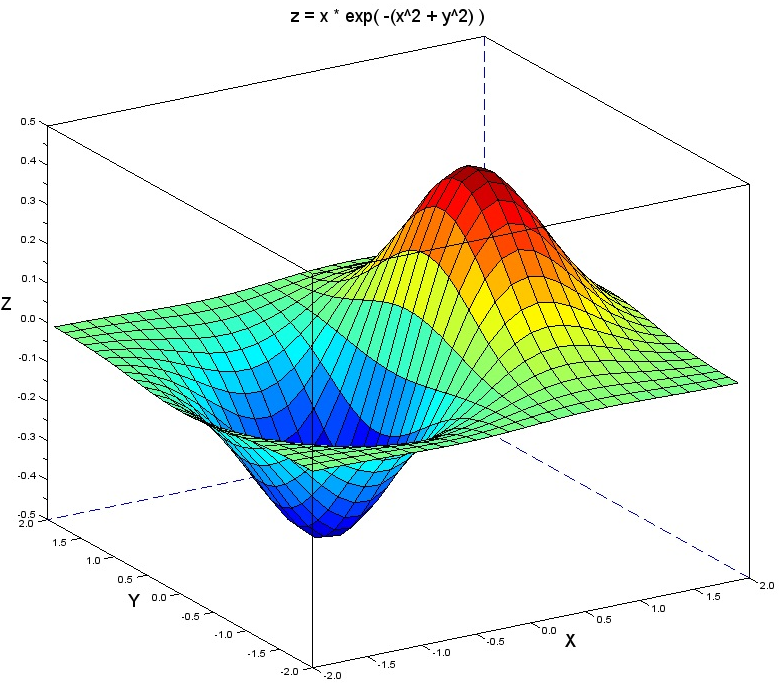
\includegraphics[width=0.7\linewidth]{./images/hw2-loss.png}
			\caption{Loss Manifold Visualization}
		\end{figure}

		Where should gradient descent end up on the graph? How many weights does this model have? If our model starts training at \( (-2, 2, 0) \), will the loss function ever reach the absolute minimum? Why? Assume the loss function at this point is \textit{perfectly flat}. (\textit{3-5 sentences})

		\vspace{0.5cm}

		\begin{solution}
			\begin{parts}
				\part Gradient descent should end up at the minimum of the graph, namely at the large hole around 0.7 on x and y.
				\part Assuming the model has no hidden layers, the model has 2 weights corresponding to the two independent variables in the graph.
				\part If the loss function is perfectly flat at \( (-2, 2, 0) \), the model will not reach the absolute minimum. This is because the gradient at this point is zero, giving no information on how to update the weights. The model will be stuck at this point indefinitely. This problem is with flat gradients is called the \textit{vanishing gradient problem}.
			\end{parts}
		\end{solution}
	\end{parts}

	\newpage

	\question We have previously worked on single-layer linear regression using one linear function:
	\[
		\mathbf{x} \mapsto \mathbf{W}_1 \mathbf{x} + \mathbf{b}_1
	\]
	mapping from \( \mathbb{R}^s \) to \( \mathbb{R}^t \). For many real-world scenarios, we actually need multiple layers to model more complex relationships.

	\begin{parts}
		\part Calculate the result after we stack another linear function
		\[
			\mathbf{x} \mapsto \mathbf{W}_2 \mathbf{x} + \mathbf{b}_2
		\]
		mapping from \( \mathbb{R}^t \) to \( \mathbb{R}^u \) right after the first one.

		\begin{solution}
			We can represent the composition of the two linear functions as
			\[
				\mathbf{x} \mapsto \mathbf{W}_2 (\mathbf{W}_1 \mathbf{x} + \mathbf{b}_1) + \mathbf{b}_2
			\]

			Expanding this, we get
			\[
				\mathbf{W}_2 \mathbf{W}_1 \mathbf{x} + \mathbf{W}_2 \mathbf{b}_1 + \mathbf{b}_2
			\]

			Thus, the result of stacking the two linear functions is
			\[
				\mathbf{W}_2 \mathbf{W}_1 \mathbf{x} + \mathbf{W}_2 \mathbf{b}_1 + \mathbf{b}_2
			\]
		\end{solution}

		\part What is the shape of \( \mathbf{W}_1, \mathbf{b}_1 \) and \( \mathbf{W}_2, \mathbf{b}_2 \)? Explain your reasoning.

		\begin{solution}
			The weights of an MLP layer are a matrix, while biases are column vectors. Following from this, if the first layer maps from \( \mathbb{R}^s \) to \( \mathbb{R}^t \), then \( \mathbf{W}_1 \) is of size \( (t, s) \) and \( \mathbf{b}_1 \) is of size \( (t, 1) \). Similarly, if the second layer maps from \( \mathbb{R}^t \) to \( \mathbb{R}^u \), then \( \mathbf{W}_2 \) is of size \( (u, t) \) and \( \mathbf{b}_2 \) is of size \( (u, 1) \).
		\end{solution}
		\part Does the composition of the two linear functions offer an improvement over a single linear function? Explain your answer (\textit{2-4 sentences}).
		\begin{solution}
			The composition of two linear functions does not offer an improvement over a single linear function, as the composition of linear functions in an ideal mathematical framework reduces to a single linear function. This is why we apply nonlinear activation functions to the output of each layer in a neural network in order to achieve higher expressiveness and describe complex systems.
			If we feel like being pedantic, we could say that the composition of two linear functions in a computationally imperfect system does offer more expressiveness due to IEEE error, but I prefer to leave that noise to the \hyperlink{http://tom7.org/grad/murphy2023grad.pdf}{PHDs}.

		\end{solution}
	\end{parts}

\end{questions}

% \section{Bonus Questions}
% 
% \begin{figure}[htbp]
% 	\centering
% 	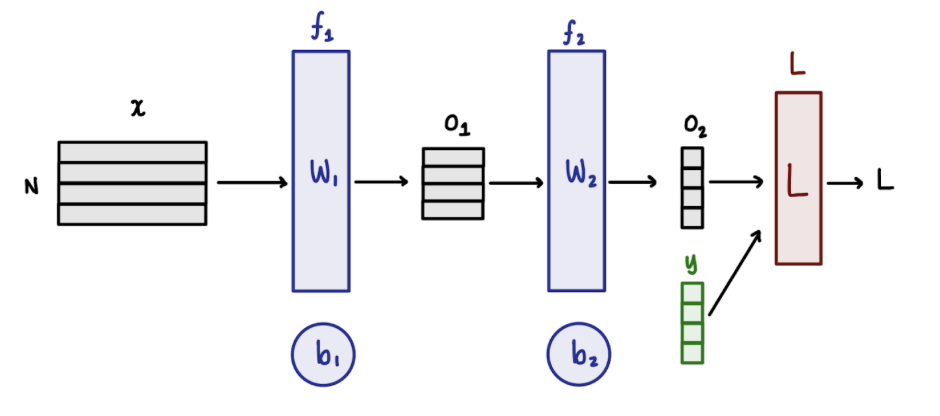
\includegraphics[width=0.7\linewidth]{./images/sample-net.png}
% 	\caption{Sample Neural Network}
% \end{figure}
% 
% For the following questions, consider the functions:
% \texttt{get\_input\_gradients()}, \texttt{get\_weight\_gradients()}, \texttt{compose\_input\_gradients()}, and \texttt{compose\_weight\_gradients()}.
% 
% \begin{questions}
% 	\question To initialize backpropagation, which function must you call on which layer? What partial derivative(s) would this return?
% 
% 	\question At layer \( f_1 \), what shape are the partials that \texttt{get\_input\_gradients(J)} and \texttt{get\_weight\_gradients(J)} return? Assume \( x \) is a vector of length \( m \) and \( w_1 \) is of size \( (m, r) \).
% 
% 	\question At layer \( f_1 \), what shape are the partials that \texttt{compose\_input\_gradients(J)} and \texttt{compose\_weight\_gradients(J)} return?
% 
% 	\question At layer \( f_1 \), how does \texttt{compose\_input\_gradients(J)} resolve the input dimension difference?
% \end{questions}
% 
% \section*{More Bonus (More Math)}
% 
% \begin{questions}
% 	\question Why don’t we use symbolic differentiation instead of gradient descent to minimize loss? (\textit{1-4 sentences})
% 
% 	\question Prove that SGD with batch size 1 gives an \textit{unbiased estimate} of the full-batch gradient.
% 
% \end{questions}
% 
\end{document}
